\documentclass[a4paper,12pt]{article}
\usepackage{styledoc19}


\begin{document} % конец преамбулы, начало документа
	
	\year{2020}
	\docNumber{RU.17701729.04.13-01 ТЗ 01-1-ЛУ}
	\docFormat{Пояснительная записка}
	\student{БПИ 174}{Д. Ю. Редникина}
	\supervisor{Профессор департамента \vfill программной инженерии  факультета компьютерных наук, к.т.н}
	{Е. М. Гринкруг}
	\project{СИСТЕМА УПРАВЛЕНИЯ ЗАДАНИЯМИ ПО АВТОМАТИЧЕСКОМУ СБОРУ ДАННЫХ ИЗ СЕТИ ИНТЕРНЕТ}
	
	\firstPage
						\newpage
	\secondPage
						\newpage
	\thirdPage
						\newpage
	\section{Введение}
	\subsection{Наименование программы}
	<<CRM-система для благотворительного фонда <<AIAIN>>. Web-приложение для сотрудников фонда>> (<<System for managing tasks of collecting data from the Internet
>>)
	
	\subsection{Документы, на основании которых ведется разработка}
	Приказ декана факультета компьютерных наук И.В. Аржанцева "Об утверждении тем, руководителей курсовых работ студентов образовательной программы «Программная инженерия» факультета компьютерных наук" № 2.3-02/1112-04 от 11.12.2019.
	\newpage
	\section{Назначение и область применения}
	\subsection{Назначение программы }
	\subsubsection{Функциональное назначение}
	Система будет применяться как средство управления проектами по созданию, редактированию и запуску веб краулеров для сбора данных в сети интернет. Продукт позволит следить за запусками в режиме реального времени, а также создавать периодические запуски по расписанию.

	\subsubsection{Эксплуатационное назначение}
	Web-приложение является компонентом CRM-системы для благотворительного фонда <<AIAIN>>, позволяющей облегчить бизнес процессы работы фонда с благополучателями и донорами. Web-приложение призвано обеспечить необходимую сотрудникам фонда функциональность для работы с системой. Им будут пользоваться как менеджеры фонда, так и администраторы, члены комиссий, операторы фонда, контент-менеджеры фонда. Каждый из пользователей будет иметь доступ к необходимой ему функциональности по обработке заявок, управлению фондом, администрированию и т.д. 
	\subsubsection{Область применения}
	Ежегодно сотни тысяч людей жертвуют свои деньги некоммерческим организациям. Еще больше людей обращаются за помощью в общественные благотворительные фонды. Управлять благотворительным фондом становится все сложнее. Нужно не только принимать пожертвования и регистрировать заявки на сборы средств, но и контролировать работников фонда, волонтеров, подготавливать документацию для вышестоящих органов и многое другое. 

Следовательно, некоммерческие организации нуждаются в платформе с функционалом, ориентированным на бизнес процессы фонда, чтобы обрабатывать всю необходимую информацию в одном месте. К сожалению, большинство фондов пользуются электронными таблицами или, что еще хуже, ведут записи в бумажной форме. Как результат, на каждое действие тратятся большое количество времени и ресурсов. Арабский фонд <<AIAIN>> также столкнулся с проблемой автоматизации бизнес процессов, специфичных для предметной области благотворительности. 


Разрабатываемое Web-приложение ориентировано на специфические нужды некоммерческой организации <<AIAIN>>. Web-приложение для сотрудников фонда может предоставить все преимущества, которыми бизнес-компании пользовались в течение многих лет и чего так не хватало этому фонду. Это также позволит наладить бизнес-процессы внутри фонда <<AIAIN>>, настроить тайм-менеджмент и автоматизировать составление отчетности.
					\newpage 
	\section{Технические характеристики}
	\subsection{Постановка задачи на разработку программы}
	Программа должна соответствовать требованиям, представленным в техническом задании:

    \newlist{subreg}{enumerate}{10}
 
\setlist[subreg, 1]{label=\textbf{FR-\arabic*.}}
\setlist[subreg, 2]{label*=\textbf{\arabic*.}}
\setlist[subreg, 3]{label=\arabic*.}

\begin{subreg}
    \item \label{FR-1} \textbf{Аутентификация\\} 
	Сотрудник фонда должен иметь возможность авторизоваться в системе с логином/паролем, предварительно полученным после регистрации по почте. Процесс регистрации и получения логина/пароля описан в пункте \ref{enum:reg}. Если пользователь не зарегистрирован в системе или авторизуется с неверными данными, то система должна отобразить соответствующее сообщение. 
	
	При первоначальном авторизации в системе на новом устройстве пользователь должен увидеть диалоговое окно с возможностью принять или отклонить получение пуш-уведомлений (подробнее о пуш-уведомлениях в разделе \ref{push}).
	
	\item \textbf{Настройки\\}
    У пользователя должна быть возможность управлять личными данными в настройках системы.
    \begin{subreg} \label{settings}
        \item Должна быть возможность просмотра информации о своем профиле в настройках системы:
        \begin{subreg}
        \item ФИО, почта;
        \item Дата рождения;
        \item Город, страна, телефон;
        \item Фотография;
        \item Роль в системе (см. Приложение \ref{stuff});
        \item Назначенные категории (только для пользователей с ролью <<Член комиссии>>);
        \end{subreg}
        \item Должна быть возможность изменения основной информации:
    \begin{subreg}
        \item ФИО;
        \item Город, страна, телефон;
        \item Фотография;
        \item Дата рождения;
    \end{subreg}
        \item Должна быть возможность выбрать язык системы: русский или английский;
        \item \label{enum:push} Должна быть возможность включить/отключить получение пуш-уведомлений; 
    \end{subreg}
    \item \textbf{Пуш-уведомления\\} \label{push}
    Сотрудники фонда должны иметь возможность получать пуш-уведомления, если такая настройка включена (см. пункт \ref{enum:push}).
    
    \begin{subreg}
        \item Должна быть возможность получения пуш-уведомлений на входящие сообщения в чатах поддержки (для пользователя с ролью <<Оператор>>, подробнее о чатах в пункте \ref{req:chats});
        
        \item Должна быть возможность получения пуш-уведомлений при изменений статусов заявок, которые назначены на конкретного менеджера (для роли <<Менеджер>> и <<Член комиссии>>, подробнее в пункте \ref{req:status});
        
        \item Должна быть возможность получения пуш-уведомлений при изменении статуса операции в системе блокчейн (подробнее в пункте \ref{req:blockchain});
        
        \item Должна быть возможность просмотра списка уведомлений и информации о них:
        \begin{subreg}
        \item Дата и время уведомления;
        \item Тип уведомления;
        \item Инициатор уведомления;
        \end{subreg}
    \end{subreg}
    
    \item \textbf{Статусы операций в системе блокчейн\\} \label{req:blockchain}
    Сотрудники фонда должны иметь возможность просматривать изменения статусов операций в системе блокчейн, а именно: дата, время совершенной операции, тип операции, статус операций, дату, время обновления статуса.
    
    \item \textbf{Управление пользователями\\}
        Этот функционал должен быть доступен только для пользователя с ролью <<Администратор>> (кроме пункта \ref{enum:managers}).
        \begin{subreg}
        \label{admin}
        \item \label{enum:admin_1} Должна быть возможность просмотра информации о пользователе: его ФИО, роль в системе, город, страна, фотография, статус в системе (заблокирован или нет), назначенные категории (только для пользователей с ролью <<Член комиссии>>);
        \item Должна быть возможность изменить все поля из пункта \ref{enum:admin_1}, кроме почты;
        
        \item \label{enum:reg} Должна быть возможность зарегистрировать пользователя в системе, указав:
        \begin{subreg}
            \item ФИО;
            \item Почту;
            \item Роль пользователя в системе (см. Приложение \ref{stuff});
            \item Назначенные категории (только для пользователей с выбранной ролью <<Член комиссии>>);
        \end{subreg}
        После совершения процесса регистрации на указанную почту пользователю приходит логин/пароль для дальнейшей аутентификации в системе;
        \item \label{enum:managers} Должна быть возможность просмотра информации о сотрудниках фонда для пользователя с ролью <<Член комиссии>>: ФИО, роль, город, страна, день рождения, телефон, назначенные категории (если есть), заявки назначенные на пользователя (если есит);
        \end{subreg}
        
    \item \textbf{Логи системы\\}
    У пользователя с ролью <<Администратор>> должна быть возможность просматривать логи системы в формате JSON с обязательными полями: дата регистрации события, тип события и также описание события.
    
    \item \textbf{Транзакции\\}
    Этот функционал должен быть доступен только для пользователя с ролью <<Член комиссии>>.
    \begin{subreg}
        \item Должна быть возможность просматривать транзакции, совершенные внутри системы, информацию о них:
    \begin{subreg}
        \item Дата, время совершения транзакции;
        \item Кто совершил транзакцию (ФИО донора);
        \item Сумма транзакции;
        \item На какую заявку транзакция была совершена - основная информация о заявке: название, автор, тип заявки;
    \end{subreg}
        \item Должна быть возможность провести ручную транзакцию -- вести данные о платеже, поступившем напрямую в фонд. При вводе транзакции должна быть возможность указать цель платежа: на одну из заявок фонда или на нужды фонда, а также ФИО пользователя от которого поступило пожертвование, сумму пожертвования;
    \end{subreg}
    
    \item \textbf{Категории\\}
    Этот функционал должен быть доступен только для пользователя с ролью <<Член комиссии>>.
    \begin{subreg}
        \item Должна быть возможность просматривать категории фонда, доступные для назначения на заявки, а именно:
        \begin{subreg}
            \item ID - уникальный идентификатор категории;
            \item Название категории на английском;
            \item Название категории на русском языке;
            \item Название категории на арабском;
            \item Видимость категории - некоторые категории должны быть скрыты от пользователей при назначении категории на заявку;
        \end{subreg}
        \item Должна быть возможность изменить все данные о категориях;
        \item Должна быть возможность удалить категорию. Для удаления доступны только те категории, которые не используются в системе (т.е не назначены на пользователей или на заявку);
    \end{subreg}
    
    \item \textbf{Заявки\\}
    Эта функциональность должна быть доступна для пользователей с ролью <<Член комисии>> и <<Менеджер>>;
    \begin{subreg}
    \item \label{req:status} Должна быть возможность изменять статусы заявок в зависимости от роли пользователя и предыдущего статуса заявки в соответствии с диаграммой жизненного цикла заявки (см. Приложение \ref{status});
    \item Должна быть возможность отредактировать данные о заявке (одобренная сумма, срок сбора средств), когда она находится в статусе <<В обработке>>; 
    \item Должна быть возможность создать заявку в системе от лица незарегистрированного пользователя. При создании заявки нужно указать: название,  описание, сумма сбора, категория заявки, документы и дата сбора. Заявка сразу создается в статусе <<Активная>> от имени фонда. Эта функциональность должна быть доступна только для пользователей с ролью <<Член комиссии>>;
    \item Должна быть возможность оставлять комментирии к заявке;
    \item Должна быть возможность просматривать комментарии к заявке: текст сообщения, дату и автора;
    \item Должна быть возможность менять менеджера, который назначен на обработку заявки;
    \item Должна быть возможность закрыть сбор средств на заявку;
    \item Должна быть возможность просмотреть информацию о голосовании по заявке в статусе <<Ждет подтверждения члена комиссии>>, а именно: кто имеет право проголосовать и их решение, а также статус голосования (в процессе, принято, отклонено);
    \item У пользователей с ролью <<Член комиссии>> должна быть возможность проголосовать по заявке (за принятие или против), если категория заявки совпадает с назначенной на члена комиссии категорией;
    \end{subreg}
    
    \item \textbf{Чаты\\} \label{req:chats}
    Данная функциональность должна быть доступна только пользователям с ролью <<Оператор>>;

    \begin{subreg}
    \item Должна быть возможность просматривать список чатов: ФИО собеседника, текст сообщения, количество непрочитанных сообщений;
    \item Должна быть возможность написать сообщение;
    \end{subreg}
    
    \item \textbf{Управление контентом фонда\\}
    Данная функциональность должна быть доступна только для пользователей с ролью <<Контент-менеджер>>;
    
    \begin{subreg}
    \item Должна быть возможность просмотривать м редактировать часто задаваемые вопросы в формате \texttt{markdown} \cite{md};
    \item Должна быть возможность просмотривать, редактировать, удалять и создавать новости фонда. Для создания нужно указать название, описание новости и фотографию;
    \item Должна быть возможность просмотра и редактирования информации о фонде: описания и загруженных документов;
    \end{subreg}
    
\end{subreg}


\renewcommand{\labelenumi}{\arabic{enumi}.}

\renewcommand{\labelenumii}{\arabic{enumii}.}

\renewcommand{\labelenumiii}{\arabic{enumiii}.}





	

Существует потребность в отслеживании информации в интернете в автоматическом режиме:
\begin{itemize}
\itemСовместное управление запусками
\itemПериодический запуск задач
\itemПросмотр логов, различных метрик
\itemБесплатная платформа
\end{itemize}

\textbf{Цель работы:}

    \begin{itemize}
        \item Разработка инструмента для управления заданиями по автоматическому сбору данных из сети Интернет
        \begin{itemize}
            \item создание запросов по созданию и запуску (в том числе и по расписанию)  краулеров
            \item предоставление запросов для доступа к данным, собираемым различными краулерами
            \item real-time мониторинг работы краулеров
            \item инфраструктура для разработки новых краулеров
        \end{itemize}
    \end{itemize}
    
\textbf{Задачи работы:}
    \begin{itemize}
        \item Разработать сервер с помощью play-framework на языке scala 
        \item Написать тесты на разрабатываемый функционал
        \item Написать техническую документацию к разрабатываемому ПО
    \end{itemize}


	\subsection{Описание алгоритмов и функционирования программы}
	\subsubsection{Описание алгоритмов программы}
	\paragraph{Алгоритм проверки наличия доступа\\ \\}
	В разрабатываемой системе практически каждый запрос имеет ограничение по доступу: изменение в проект могут вносить только участники с \texttt{ReadAndWrite} или \texttt{Owner} доступом, \texttt{ProjectId} и \texttt{CrawlerId} для запуска должны совпадать, удалять проект может человек с \texttt{Owner} правами и т.д.
	
	Для обработки таких ситуаций было принято решение создать \texttt{SecurityService}, который реализовывает алгоритм работы с несколькими проверками сразу и обработкой ошибок доступа.
	
	Была реализована функция выполнения \textit{nextAction} - следующего действия в базе данных по результату предыдущей \ref{lst:func}. С помощью функции \textt{flatMap} можно делать композицию функции и таким образом соединять несколько проверок в единое целое. \cite{flatmap} 
	
	Целью данного механизма было желание добиться легкого в изменении способа проверки нескольких условий одновременно с выводом читабельной ошибки, если где-то в середине что-то пойдет не так.
	
	\begin{lstlisting}[frame=single, basicstyle=\footnotesize\ttfamily, label={lst:func}, caption={Нестинг функций},captionpos=b]
        accessRight(ReadAndWrite) >> jobToProject >> jobToStatus(Running) 
	\end{lstlisting}
	
	На примере \textt{JobsController} можно увидеть, как легко использовать такой механизм для проверки нескольких условий.
	
	\begin{lstlisting}[frame=single, basicstyle=\footnotesize\ttfamily, label={lst:func}, caption={Функция для проверки доступа пользователя и запуска},captionpos=b]
def checkUserProjectAndJob(userId: UUID,
                             projectId: Long,
                             jobId: Long,
                             userAccess: MembershipAccessRight = Readonly):
                             Future[Option[JobExecution]] = {

    val jobExecutionAction =
      hasPermissionToAccessProject(projectId, userId, userAccess)
      .flatMap(checkResultAndPerformNextAction(
            SecurityService.UserAccessMessage, 
            jobExecCorrespondsToProject(projectId, jobId)))
      .flatMap(res => checkResultAndPerformNextAction(
            SecurityService.JobExecutionToProjectMessage, 
            DBIO.successful(res))(res))

    db.run(jobExecutionAction)
  }
	\end{lstlisting}
	
	\subsubsection{Описание схемы функционирования программы}
	
	Диаграмма вариантов использования (\ref{pic: usecase}) отображает ключевые преценденты и главных акторов системы. Первостепенный актор - обычный пользователь, описание и профиль которого представлены в разделах \ref{subsub: userprofile} и \ref{subsub: userlist}. Второстепенные акторы системы - база данных postgres \cite{postgresql}, а также scrapyd \cite{scrapyd}. Вот основные преценденты, которые инициирует обычный пользователь в рамках системы :
	\begin{enumerate}
	    \item Авторизация;
	    \item \textbf{CRUD работ по запуску};
	    \label{g:CRUDjobs}
	    \item CRUD периодических задач;
	    \item Просмотр и редактирование пауков;
	    \item \textbf{CRUD проектов};
	    \label{g:CRUDprojects}
	\end{enumerate}
	
Преценденты \ref{g:CRUDprojects} и \ref{g:CRUDjobs} будут расмотрены детально в этом разделе на странице \pageref{s: spec}.  Область применения разрабатываемой системы продемонстрирована на рисунке \ref{pic: classdiagram}. 
	
	\begin{figure}[H]
		\centering
		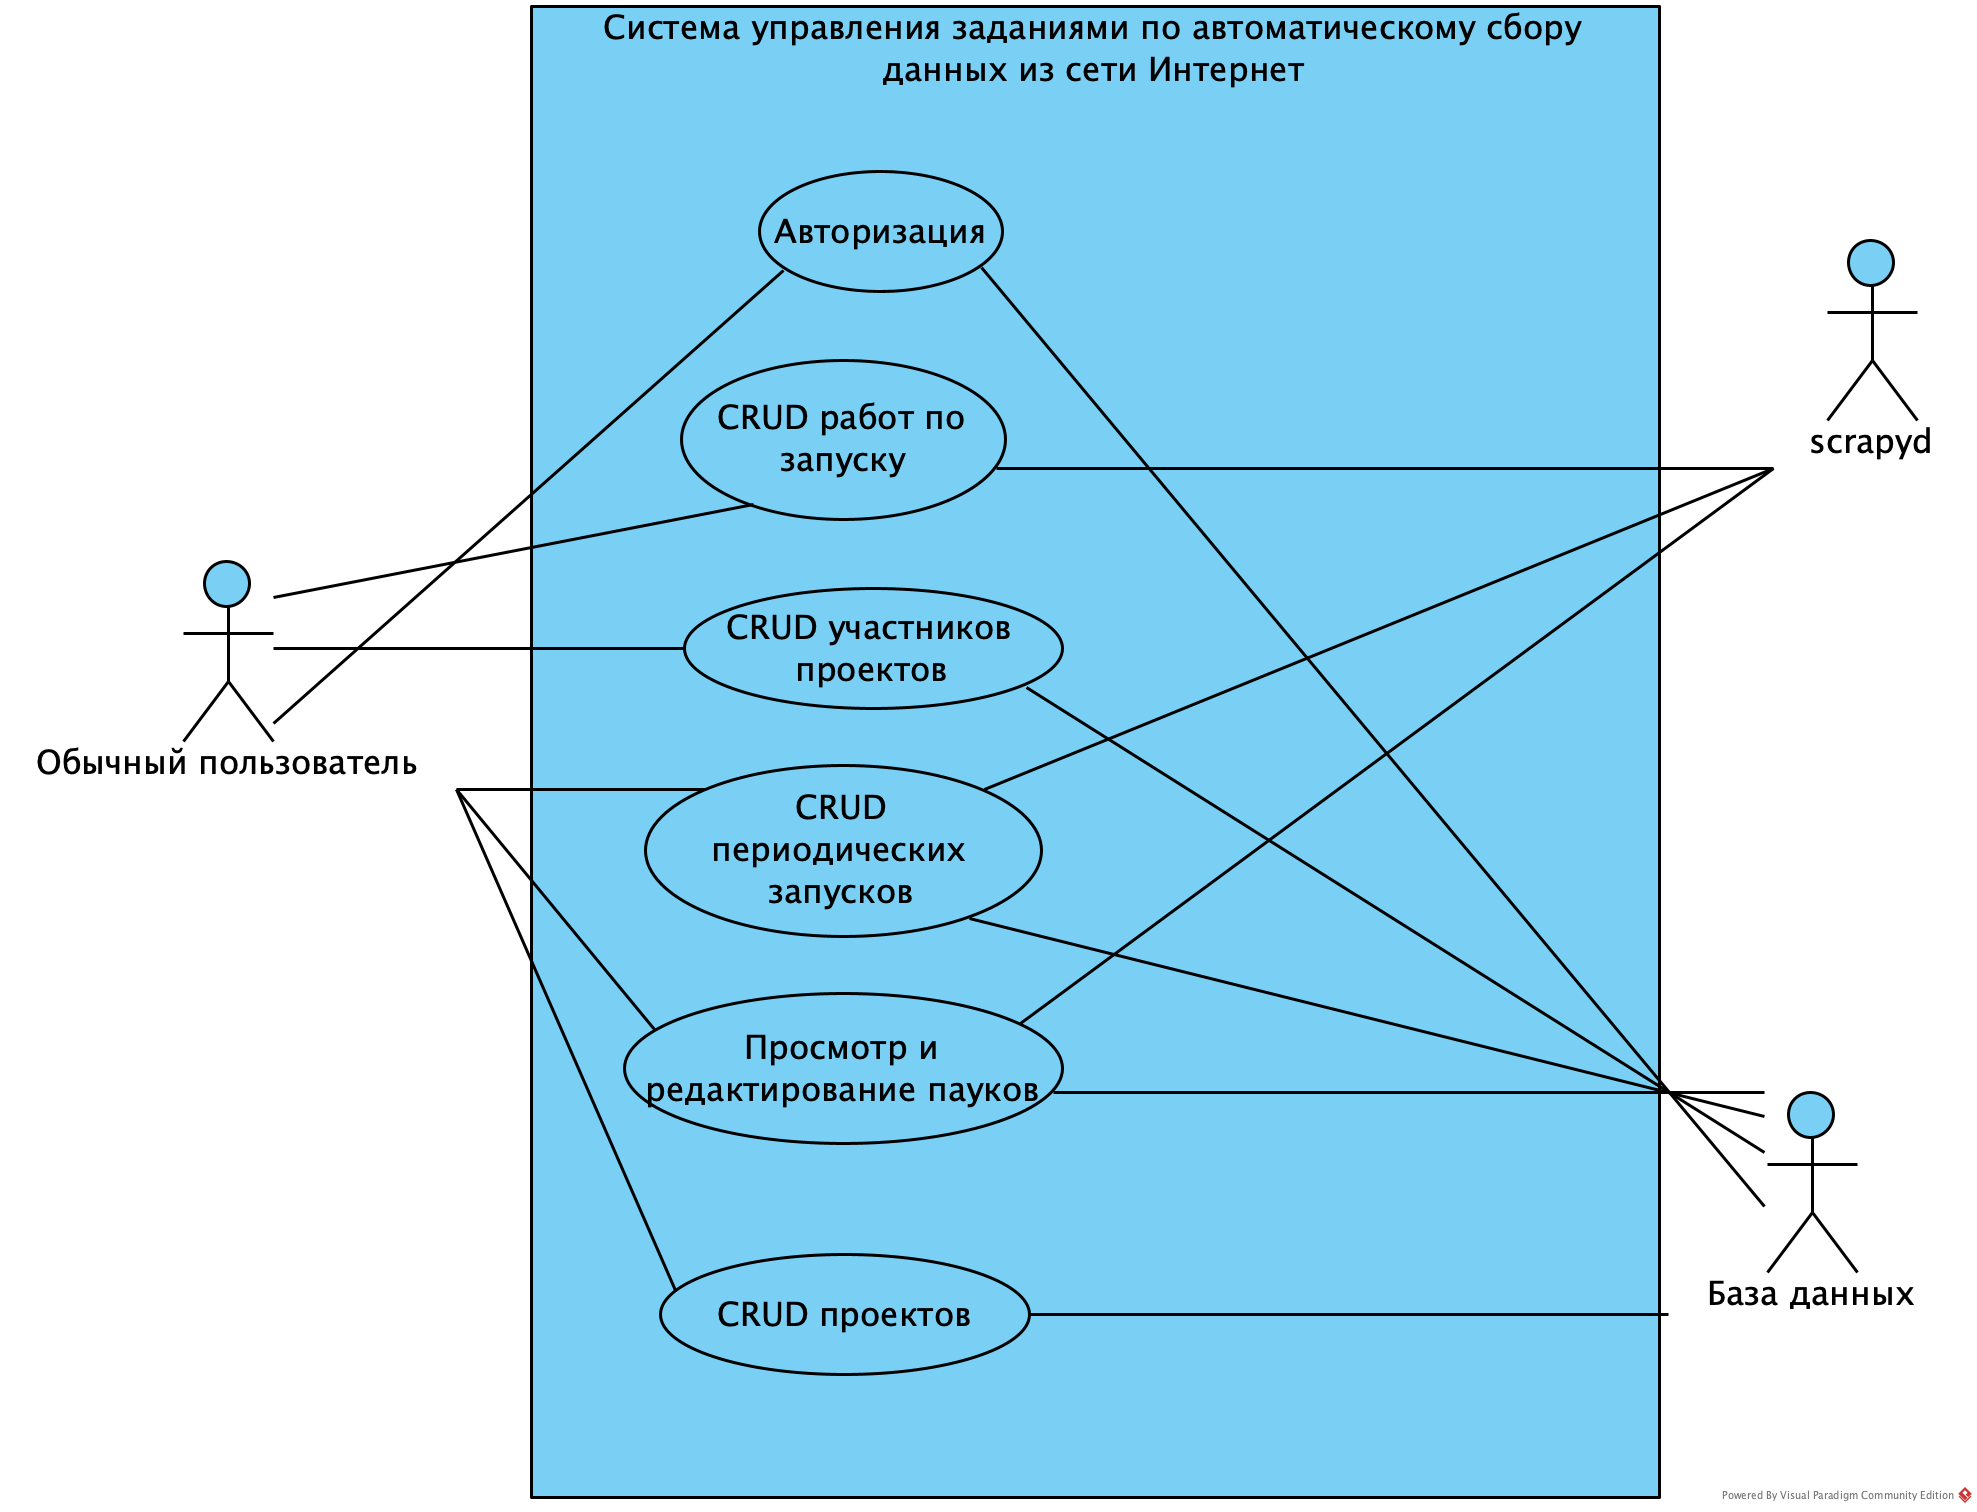
\includegraphics[width = 0.8\linewidth]{img/uml/UseCase.png}
		\caption{Use-case диаграмма}
		\label{pic: usecase}
	\end{figure}
	
	\begin{figure}[h]
		\centering
		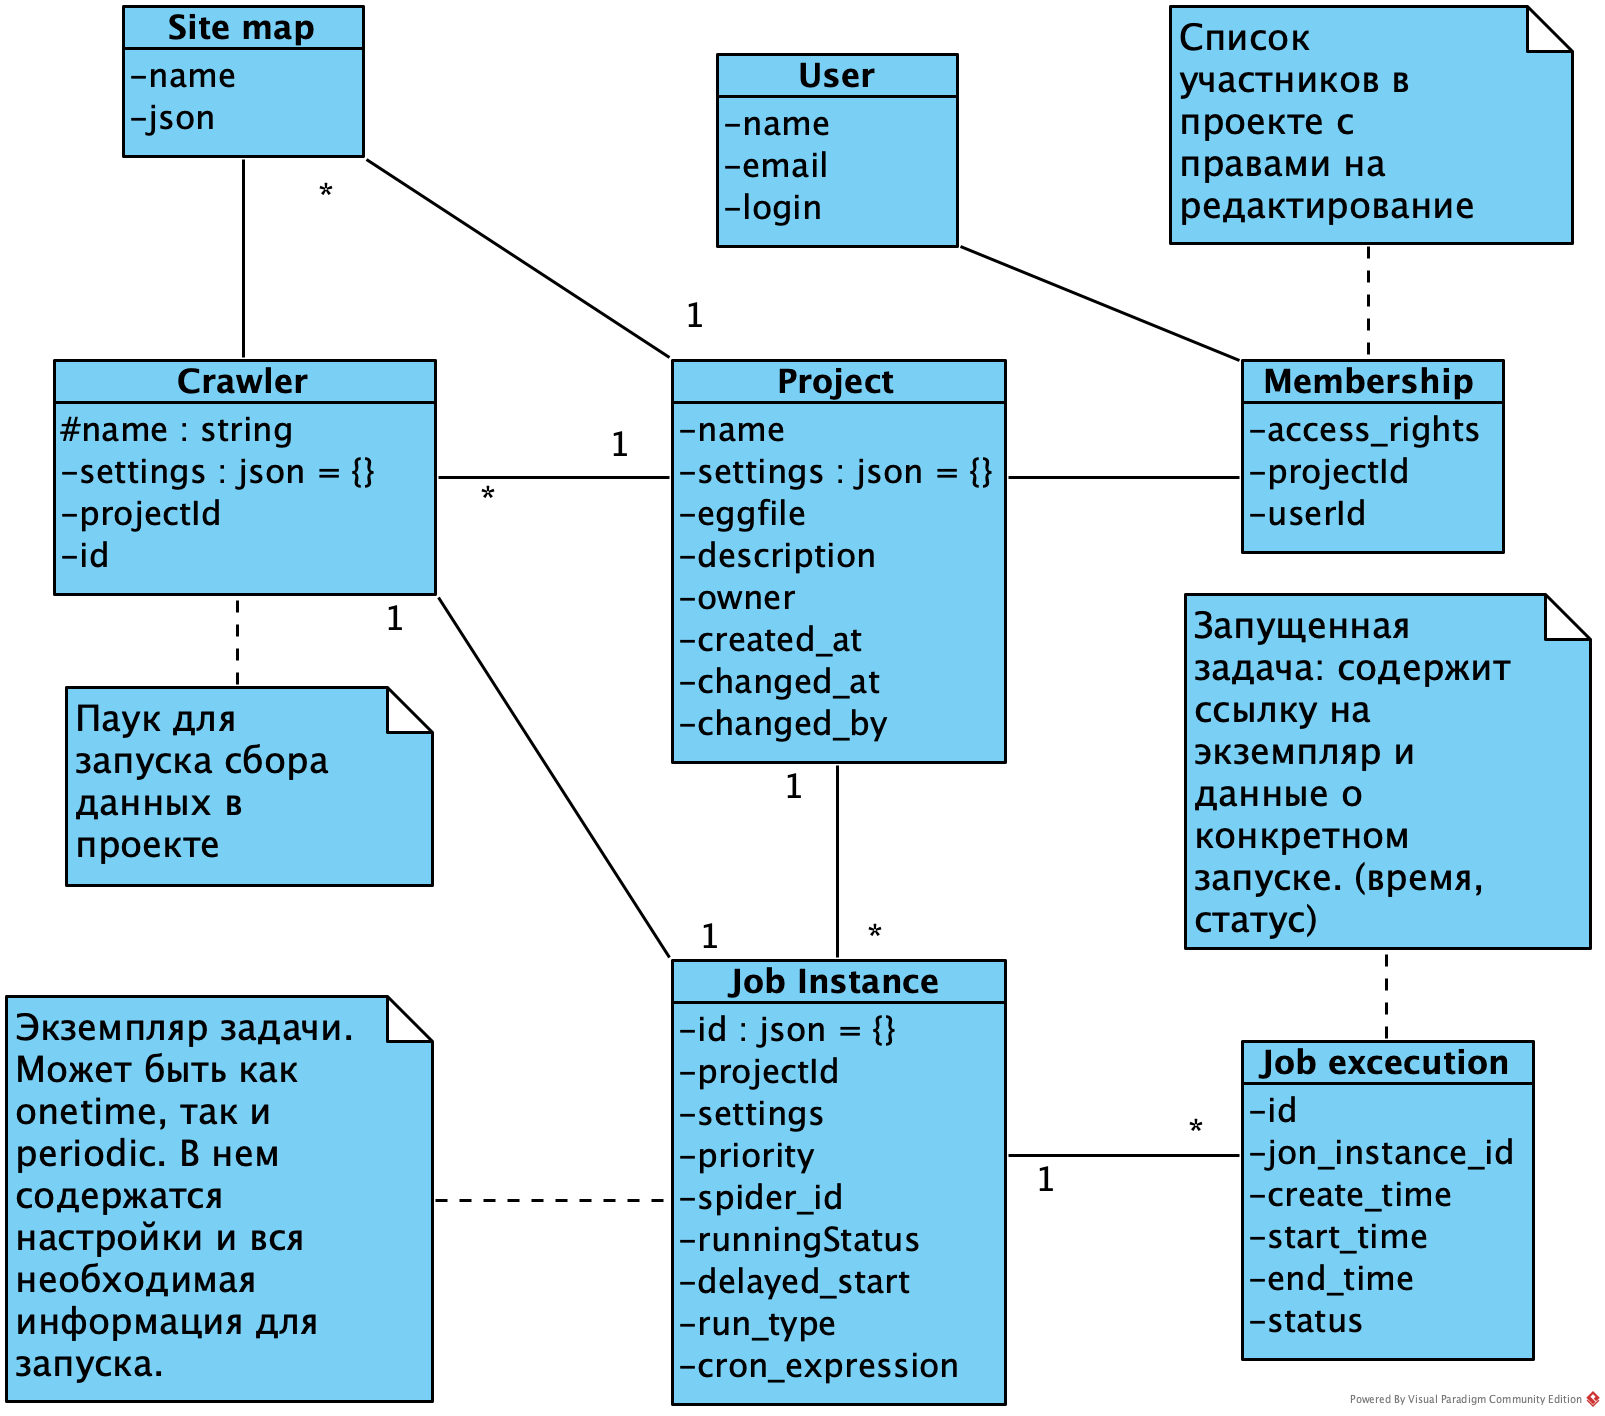
\includegraphics[width = 0.8\linewidth]{img/ClassDiagram.png}
		\caption{Диаграмма области применения}
		\label{pic: classdiagram}
	\end{figure}
	
	приетв
	
	
	\section*{Спецификации прецендентов} \label{s: spec}
	
	\subsection*{Спецификация прецендента <<CRUD запусков>>}
	
	\begin{longtable}[]{|@{\textbf}r|p{7cm}|} 
    \caption{Краткая информация о преценденте}
    \hline
    Название             & <<CRUD запусков>>   \\ \hline
    Аннотация            & Любой пользователь, имеющий доступ к проекту \texttt{Owner} или \texttt{ReadAndWrite}, может создать запуск из имеющихся в проекте краулеров. Запуск может иметь приоритет, а также настройки и аргументы для скрейпинга. В результате запуска пользователю будут доступны логи и результаты сбора. \\ \hline
    Автор документа      & Редникина Д.Ю.     \\ \hline
    Рамки применения     & Вся система     \\ \hline
    Уровень              & Ключевая задача                     \\ \hline
    Основной исполнитель & Обычный пользователь     \\ \hline
\end{longtable}

\subsection*{Основной поток}

\begin{enumerate}
    \item Пользователь начинает прецендент: отправляет запрос на просмотр данных о задачах в статусе \texttt{finished}.
    \item Система формирует JSON со списком задач в статусе \texttt{finished}, к которым у пользователя есть доступ.
    \item Пользователь отправляет запрос на создание нового запуска, при этом указав id паука для запуска, приоритетность запуска, фргументы и настройки для запуска. Данные должны быть в формате JSON \ref{lst:POSTjob}. \label{g:createjob}
    \item Система валидирует полученные данные.
    \item Система отправляет запрос на scrapyd для создания запуска.
    \item Система создает новый запуск в статусе \texttt{pending} в базе данных.
    \item Система формирует JSON с созданным запуском и информацией о нем.
\end{enumerate}

\subsection*{Альтернативные потоки}

\subsection*{Альтернативный поток 1}

\paragraph*{Условие начала} В шаге \ref{g:createjob} основного потока пользователь отправил JSON в неверном формате. 

\begin{enumerate}
    \def\labelenumi{\arabic{enumi}.}
    \item Система валидирует данные.
    \item Система возвращает статус-код \texttt{BAD\_REQUEST} с сообщением об неверном формате введенных данных. 
\end{enumerate}

\subsection*{Альтернативный поток 2}

\paragraph*{Условие начала} В шаге \ref{g:createjob} основного потока пользователь отправил запрос на создание запуска с краулером, находящимся в проекте id, к которому пользователь имеет доступ \texttt{ReadOnly}.

\begin{enumerate}
    \item Cистема валидирует права доступа пользователя к проекту id.
    \item Система возвращает статус-код \texttt{FORBIDDEN} с сообщением <<You don't have permission to run a job>>.
\end{enumerate}

\subsection*{Альтернативный поток 3}

\paragraph*{Условие начала} В шаге \ref{g:createjob} пользователь отправляет \texttt{CrawlerId} паука, для которого хочет совершить запуск и \texttt{ProjectId} проекта, к которому имеет \texttt{Owner} или \texttt{ReadAndWrite} доступ. Паука с \texttt{CrawlerId} нет в проекте \texttt{ProjectId}.

\begin{enumerate}
    \item Система валидирует права доступа к проекту и наличие паука в проекте с данным \texttt{projectId}.
    \item Система возвращает статус-код \texttt{FORBIDDEN} с сообщением <<Project and crawler doesn't match>>.
\end{enumerate}

\subsection*{Альтернативный поток 4} 
\paragraph*{Условие начала} На шаге \ref{g:createjob} пользователь отправляет запрос на отмену запуска \texttt{id}, который находится в статусе \texttt{Pending} или \texttt{Running}.

\begin{enumerate}
    \item Система валидирует данные: доступ пользователя к отмене задачи, а также статус задачи.
    \item Система отправляет запрос на \texttt{scrapyd} для отмены запущенной задачи.
    \item Система валидирует полученный результат.
    \item Система изменяет статус задачи на \texttt{Finished}.
    \item Система отправляет статус-код \texttt{OK} и \texttt{id} отмененной задачи.
\end{enumerate}


\subsection*{Альтернативный поток 5} 
\paragraph*{Условие начала} На шаге \ref{g:createjob} пользователь отправляет запрос на отмену запуска \texttt{id}, который находится в статусе \texttt{Finished}.

\begin{enumerate}
    \item Система валидирует данные: доступ пользователя к отмене задачи, а также статус задачи.
    \item Система возвращает статус-код \texttt{FORBIDDEN} с сообщением <<Job has already finished>>.
\end{enumerate}


\subsection*{Альтернативный поток 6} 
\paragraph*{Условие начала} На шаге \ref{g:createjob} пользователь отправляет запрос на удаление запуска \texttt{id}, который находится в статусе \texttt{Finished}.

\begin{enumerate}
    \item Система валидирует данные: доступ пользователя к отмене задачи, а также статус задачи.
    \item Cистема удаляет данные о задаче в базе данных.
    \item Система возвращает статус-код \texttt{OK}.
\end{enumerate}

\subsection*{Альтернативный поток 7} 
\paragraph*{Условие начала} На шаге \ref{g:createjob} пользователь отправляет запрос на удаление запуска \texttt{id}, который находится в статусе \texttt{Pending} или \texttt{Running}.

\begin{enumerate}
    \item Система валидирует данные: доступ пользователя к отмене задачи, а также статус задачи.
    \item Система возвращает статус-код \texttt{FORBIDDEN} с сообщением <<Job is not in finished state>>.
\end{enumerate}


\begin{longtable}[]{|@{\textbf}r|p{7cm}|} 
\caption{Пред- и постусловия для прецендента}
\hline
    Предусловия            &  Пользователь авторизован в системе. \\ \hline
    Постусловия            & В системе зафиксированы совершенные запуски.              \\ \hline
    Специальные требования & Пользователь должен быть знаком с технологией web-scraping. \\ \hline
    Список технологий      & База данных Postgresql. Scrapyd. \\ \hline
    Приоритет              & Высокий \\ \hline
    Открытые проблемы      &            \\ \hline
\end{longtable}

\clearpage
	
	\subsection*{Спецификация прецендента <<CRUD проектов>>}
	
	\begin{longtable}[]{|@{\textbf}r|p{7cm}|} 
    \caption{Краткая информация о преценденте}
    \hline
    Название             & <<CRUD проектов>>   \\ \hline
    Аннотация            & Любой пользователь системы имеет возможность создать проект. Проект - это сущность для организации краулеров, а также их запусков и периодических задач в одно целое. Над проектом может работать как один человек, так и несколько. \\ \hline
    Автор документа      & Редникина Д.Ю.     \\ \hline
    Рамки применения     & Вся система     \\ \hline
    Уровень              & Ключевая задача                     \\ \hline
    Основной исполнитель & Обычный пользователь     \\ \hline
\end{longtable}

\subsection*{Основной поток}

Диаграмма базового потока представлена на рисунке \ref{pic:baseflow-projects}.

\begin{enumerate}
    \def\labelenumi{\arabic{enumi}.}
    \item Пользователь начинает прецендент.
    \item Система формирует JSON со списком проектов, к которым у пользователя есть доступ. \label{g:start}
    \item Пользователь отправляет запрос на создание нового проекта, при этом указав название и опциональное описание проекта. Данные должны быть в формате JSON \ref{lst:POST}. \label{g:create}
    \item Система валидирует полученные данные (название и описание проекта).
    \item Система создает новый проект с указанными данными и присваивает пользователю \texttt{Owner} права на доступ к проекту.
    \item Система формирует JSON с созданным проектом и информацией о нем.
    \label{g:end}
\end{enumerate}






\subsection*{Альтернативные потоки}

\subsection*{Альтернативный поток 1}

\paragraph*{Условие начала} В шаге \ref{g:create} основного потока пользователь отправил JSON в неверном формате.

\begin{enumerate}
    \def\labelenumi{\arabic{enumi}.}
    \item Система валидирует данные.
    \item Система возвращает статус-код \texttt{BAD\_REQUEST} с сообщением об неверном формате введенных данных. 
\end{enumerate}

\subsection*{Альтернативный поток 2}

\paragraph*{Условие начала} В шаге \ref{g:create} основного потока пользователь отправляет запрос об изменении одного из вернувшихся на предыдущем шаге \ref{g:start} проекта. Пользователь имеет \texttt{ReadAndWrite} права на редактирование этого проекта.

\begin{enumerate}
    \def\labelenumi{\arabic{enumi}.}
    \item Пользователь отправляет JSON с данными, которые должны быть изменены о проекте, в формате \ref{lst:PUT} или \ref{lst:DEPLOY}. 
    \item Система валидирует доступ пользователя к изменяемому проекту и данные.
    \item Система фиксирует внесенные пользователем изменения.
    \item Система отображает статус-код операции \texttt{OK}.
\end{enumerate}

\subsection*{Альтернативный поток 3}

\paragraph*{Условие начала} В шаге \ref{g:create} основного потока пользователь отправляет запрос об изменении одного из вернувшихся на предыдущем шаге \ref{g:start} проекта. Пользователь имеет \texttt{ReadOnly} права на редактирование этого проекта.

\begin{enumerate}
    \def\labelenumi{\arabic{enumi}.}
    \item Пользователь отправляет JSON с данными, которые должны быть изменены о проекте, в формате. 
    \item Система валидирует доступ пользователя к изменяемому проекту и данные.
    \item Система возвращает статус-код операции \texttt{FORBIDDEN} с сообщением <<You don't have permission to change project>>.
\end{enumerate}

\subsection*{Альтернативный поток 4}

\paragraph*{Условие начала} В шаге \ref{g:create} основного потока пользователь отправляет запрос об удалении проекта. У пользователя \texttt{Owner} доступ к проекту.

\begin{enumerate}
    \def\labelenumi{\arabic{enumi}.}
    \item Пользователь отправляет запрос с \texttt{id} проекта, который хочет удалить.
    \item Система валидирует права доступа к проекту и наличие проекта с данным \texttt{id}.
    \item Система удаляет проект из БД.
    \item Система возвращает статус-код \texttt{OK}.
\end{enumerate}

\subsection*{Альтернативный поток 5}

\paragraph*{Условие начала} В шаге \ref{g:create} основного потока пользователь отправляет запрос об удалении проекта. У пользователя \texttt{ReadOnly} или \texttt{ReadAndWrite} доступ к проекту.

\begin{enumerate}
    \def\labelenumi{\arabic{enumi}.}
    \item Пользователь отправляет запрос с \texttt{id} проекта, который хочет удалить.
    \item Система валидирует права доступа к проекту и наличие проекта с данным \texttt{id}.
    \item Система возвращает статус-код \texttt{FORBIDDEN} с сообщением <<You don't have permission to delete project>>.
\end{enumerate}

\subsection*{Альтернативный поток 6}

\paragraph*{Условие начала} В шаге \ref{g:create} основного потока пользователь отправляет запрос об удалении проекта. У пользователя могут быть любые права доступа.

\begin{enumerate}
    \def\labelenumi{\arabic{enumi}.}
    \item Пользователь отправляет запрос с \texttt{id} проекта, который хочет удалить.
    \item Система валидирует права доступа к проекту и наличие проекта с данным \texttt{id}.
    \item Система возвращает статус-код \texttt{FORBIDDEN} с сообщением <<Project doesn't exist>>.
\end{enumerate}


\begin{longtable}[]{|@{\textbf}r|p{7cm}|} 
\caption{Пред- и постусловия для прецендента}
\hline
    Предусловия            &  Пользователь авторизован в системе. \\ \hline
    Постусловия            & В системе зафиксированы произведенные изменения проектов.                                                                          \\ \hline
    Специальные требования & Пользователь должен быть знаком с технологией web-scraping. \\ \hline
    Список технологий      & База данных Postgresql.   \\ \hline
    Приоритет              & Высокий \\ \hline
    Открытые проблемы      &                                                                                                                                    \\ \hline
\end{longtable}


\begin{figure}[H]
		\centering
		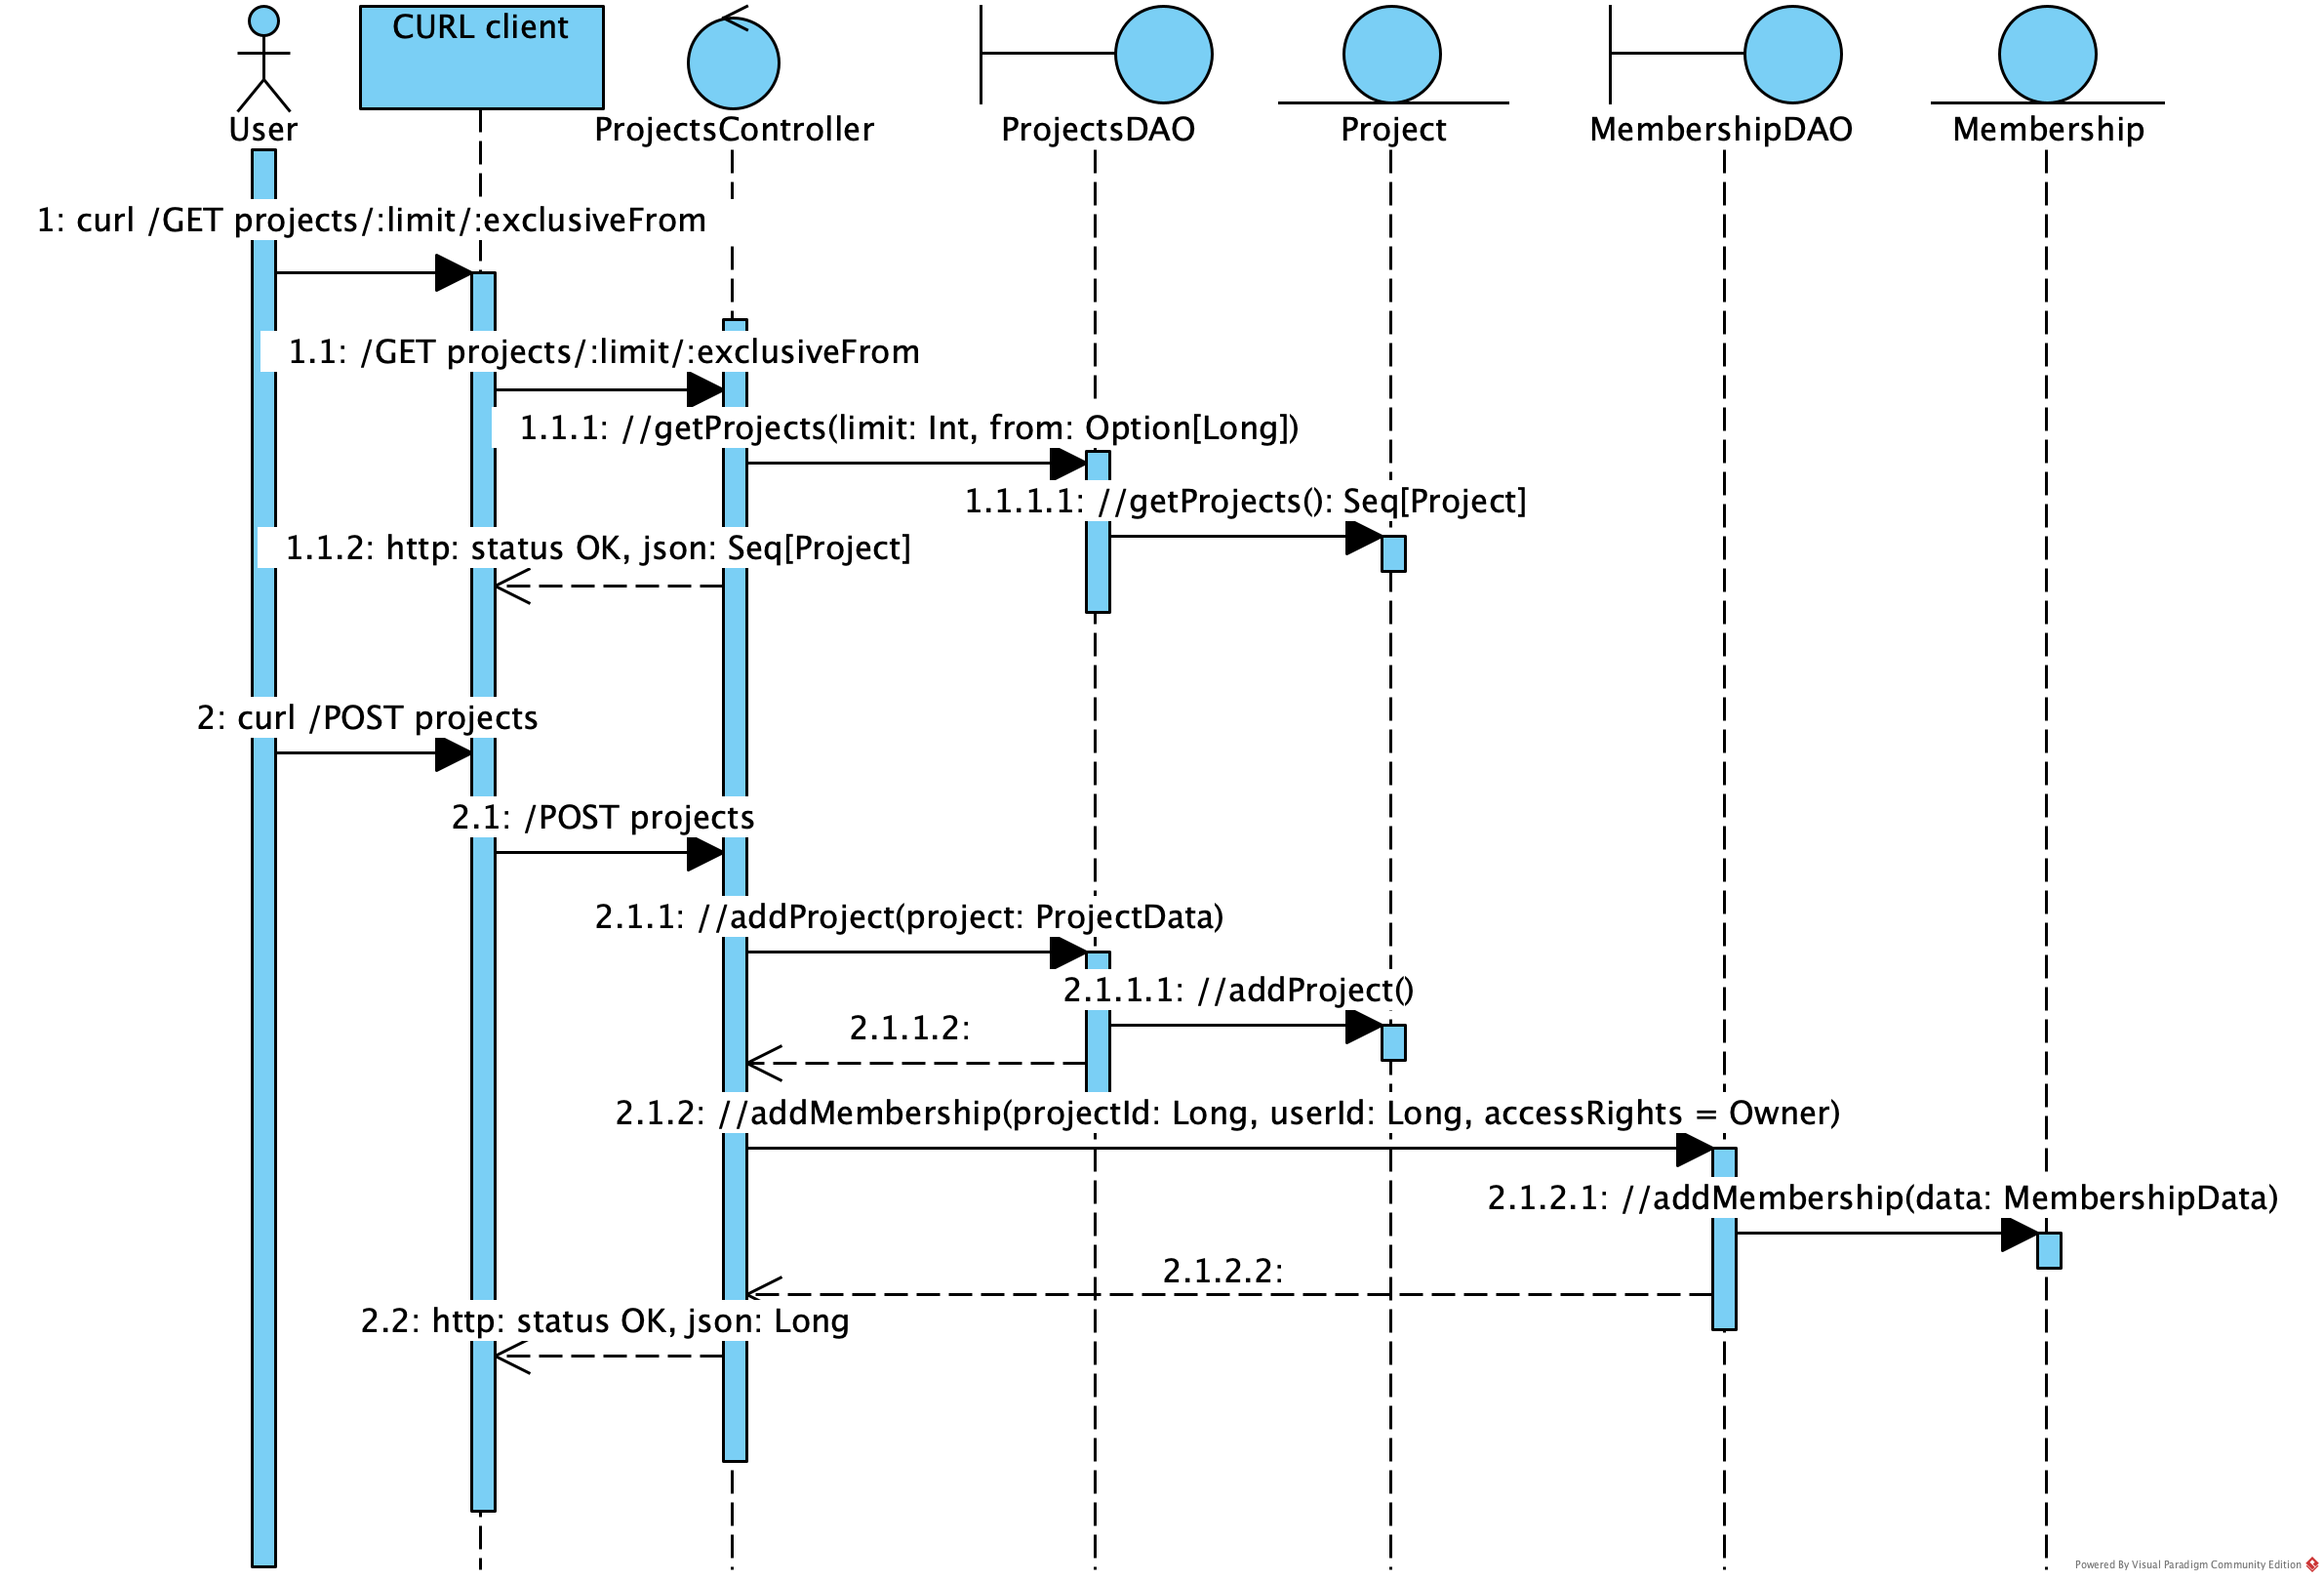
\includegraphics[width = \linewidth]{img/BaseFlow-Projects.png}
		\caption{Базовый поток прецендента <<CRUD проектов>>}
		\label{pic:baseflow-projects}
	\end{figure}




	
	
	
	
\clearpage
	\subsubsection{Возможные взаимодействия программы с другими программами}
	
	Разрабатываемая программа взаимодействует с scrapyd \cite{scrapyd}. Базовый функционал этого сервера используется для непосредственного запуска пауков.
	\subsection{Описание и обоснование выбора метода организации входных и выходных данных}

	
	Так как разрабатываемая программа является серверным приложением, то для формата входных данных был выбран JSON формат. Такая организация ввода позволяет быстро производить ввод данных, и препятствует ошибочному и некорректному заполнению данными полей базы данных.
	
	Для организации выходных данных также был выбран JSON формат. Это позволяет клиентам легко интерпретировать и отображать данные, так как JSON - самый популярный формат для сериализации передаваемых данных в клиент-серверных приложениях \cite{json}.
	\subsection{Описание и обоснование выбора состава технических и программных средств}
	\subsubsection{Состав технических и программных средств}
	При разработке программного продукта использовались следующие технические и программные средства:
	\begin{itemize}
		\item Язык разработки: Scala 2.13.1
		\item Фреймворк: Play-framework 2.6.13 \cite{play}
		\item Среда разработки: IntelliJ IDEA 2019.2 (Ultimate Edition)
		\item Dependency manager: sbt
		\item MacBook (Retina, 12-inch, Early 2016)
		\item Операционная система: macOS Catalina Version 10.15.2
		\item Библиотеки, использованные при разрабоке: 
		\begin{itemize}
			\item play-silhouette 5.0.3
			\item postgresql 42.2.8
			\item play-slick 3.0.1
			\item slick-pg 0.18.0
			\item slick-pg\_play-json 0.18.0
			\item scala-guice 4.2.6
			\item swagger-play2 1.6.1
			\item scalacheck 1.13.5
			\item scalatestplus-play 3.1.2
			\item akka-quartz-scheduler 1.8.2-akka-2.6.x
		\end{itemize}
	\end{itemize}

	\subsubsection{Обоснование выбора библиотек}
	
	\paragraph{slick / play-slick / slick-pg\\ \\}
	
	Slick - это современная библиотека для совершения запросов к базе данных и доступа к ней, реализованная на языке Scala. Она позволяет работать с данными из БД почти так же, как если использовать коллекции из стандартной библиотеки Scala, и в то же время дает полный контроль над тем, когда происходит доступ к базе данных и какие данные передаются. Преимущество библиотеки заключается в том, что можно писать запросы к базе данных на type-safe Scala вместо SQL, получая таким образом статическую проверку совместимости типов, безопасность во время компиляции и композиционность в Scala. Также в Slick есть расширяемый компилятор запросов, который может генерировать код для разных бэкэндов. 
	
	Play-slick - это библиотека, которая позволяет интегрировать Slick \cite{slick} в жизеннный цикл приложения в Play-framework \cite{play}, а также поддерживает play-эволюции \footnote{Эволюции не использовались при разработки системы}.
	
	Slick-pg - надстройка над Slick \cite{slick}, которая позволяет работать с Jsonb типом и enum в Postgresql \cite{postgresql}.
	
	\paragraph{play-silhouette \% tests\\ \\}
	Библиотека \textt{Silhouette} - это библиотека аутентификации для приложений Play Framework \cite{play}, которая поддерживает несколько методов аутентификации, включая OAuth1, OAuth2, OpenID, CAS, Credentials, Basic Authentication или пользовательские схемы аутентификации \cite{silhouette}. При проектировании приложения было принято решение использовать механизм аутентификации через Cookie - библиотека прекрасно подошла. Более того, существует удобный механизм для тестирования api-запросов, написанный с помощью \texttt{SecuredActions} библиотеки Silhouette - Silhouette-Testing. Также библиотека поддерживает механизм авторизациии через социальные сети - таким образом в будущем при расширении функционала приложения можно будет легко встроить механизм такой авторизации. \cite{silhouette-testing}. 
	
	\paragraph{akka-quartz-scheduler\\ \\}
	
	Для запуска периодических задач были рассмотрены следующие библиотеки, подходящие для использования в Play-framework \cite{play}. Основное требование к библиотеке - запуски по cron-expression на долговременный период.
	
	\begin{longtable}[]{|>{\bfseries}l| p{5cm}|p{5cm}|} 
\caption{Рассмотренные библиотеки для периодического запуска}
\hline
\textbf{Библиотека} & \textbf{Плюсы} & \textbf{Минусы} \\ \hline
    Scala's tasks            & Поддерживается & The Akka Scheduler не предназначен для использования на длительные периоды запусков, также не гарантирована точность запусков. \\ \hline
    Monix + cron4s           & Хорошая и популярная библиотека. & Очень много зависимостей. Пришлось бы писать много кода для соединения с cron4s. \\ \hline
    akka-quartz-scheduler    &  Иделаьно подходит под задачи проекта. Есть работа с cron-expression. & Не работает на более новых версиях Play-framework \cite{play} (> 2.6.13)\\ \hline
    fs2      & Библиотека для асинхронных запусков в функциональном стиле. & Не предназначена для данного вида задач, придется писать обертку. Нет работы с cron-expression.  \\ \hline
    play-akkjobs       &  На официальном сайте Play-framework ссылка на эту библиотеку как на хороший scheduler & Не поддерживается \\ \hline
\end{longtable}
	
	По итогам сравнения была выбрана библиотека \textt{akka-quartz-scheduler}.
	\subsubsection{Обоснование выбора языка программирования}
	\paragraph{Scala\\ \\}
	
	Scala объединяет объектно-ориентированное и функциональное программирование в одном емком языке высокого уровня. Статические типы Scala помогают избежать ошибок в сложных приложениях, а среда выполнения JVM  позволяет создавать высокопроизводительные системы с легким доступом к огромным экосистемам библиотек.
	
	\subsubsection{Обоснование выбора шаблона проектирования}
	\paragraph{MVC\\ \\}
	Так как разработка велась в фреймворке Play \cite{play}, то был использован подход с паттерном MVC \cite{play-mvc} для работы с HTTP-запросами. MVC представляет Controllers, Views\footnote{Так как разрабатывалось серверное приложение, то views не использовались}, Actions - для работы с api-запросами.
	\paragraph{Слоистая архитектура проектирования\\ \\}
	
	При разработке использовался архитектурный подход - layers. Все приложение поделено на несколько слоев (см. рисунок \ref{pic:layers})
	
	\begin{figure}[H]
		\centering
		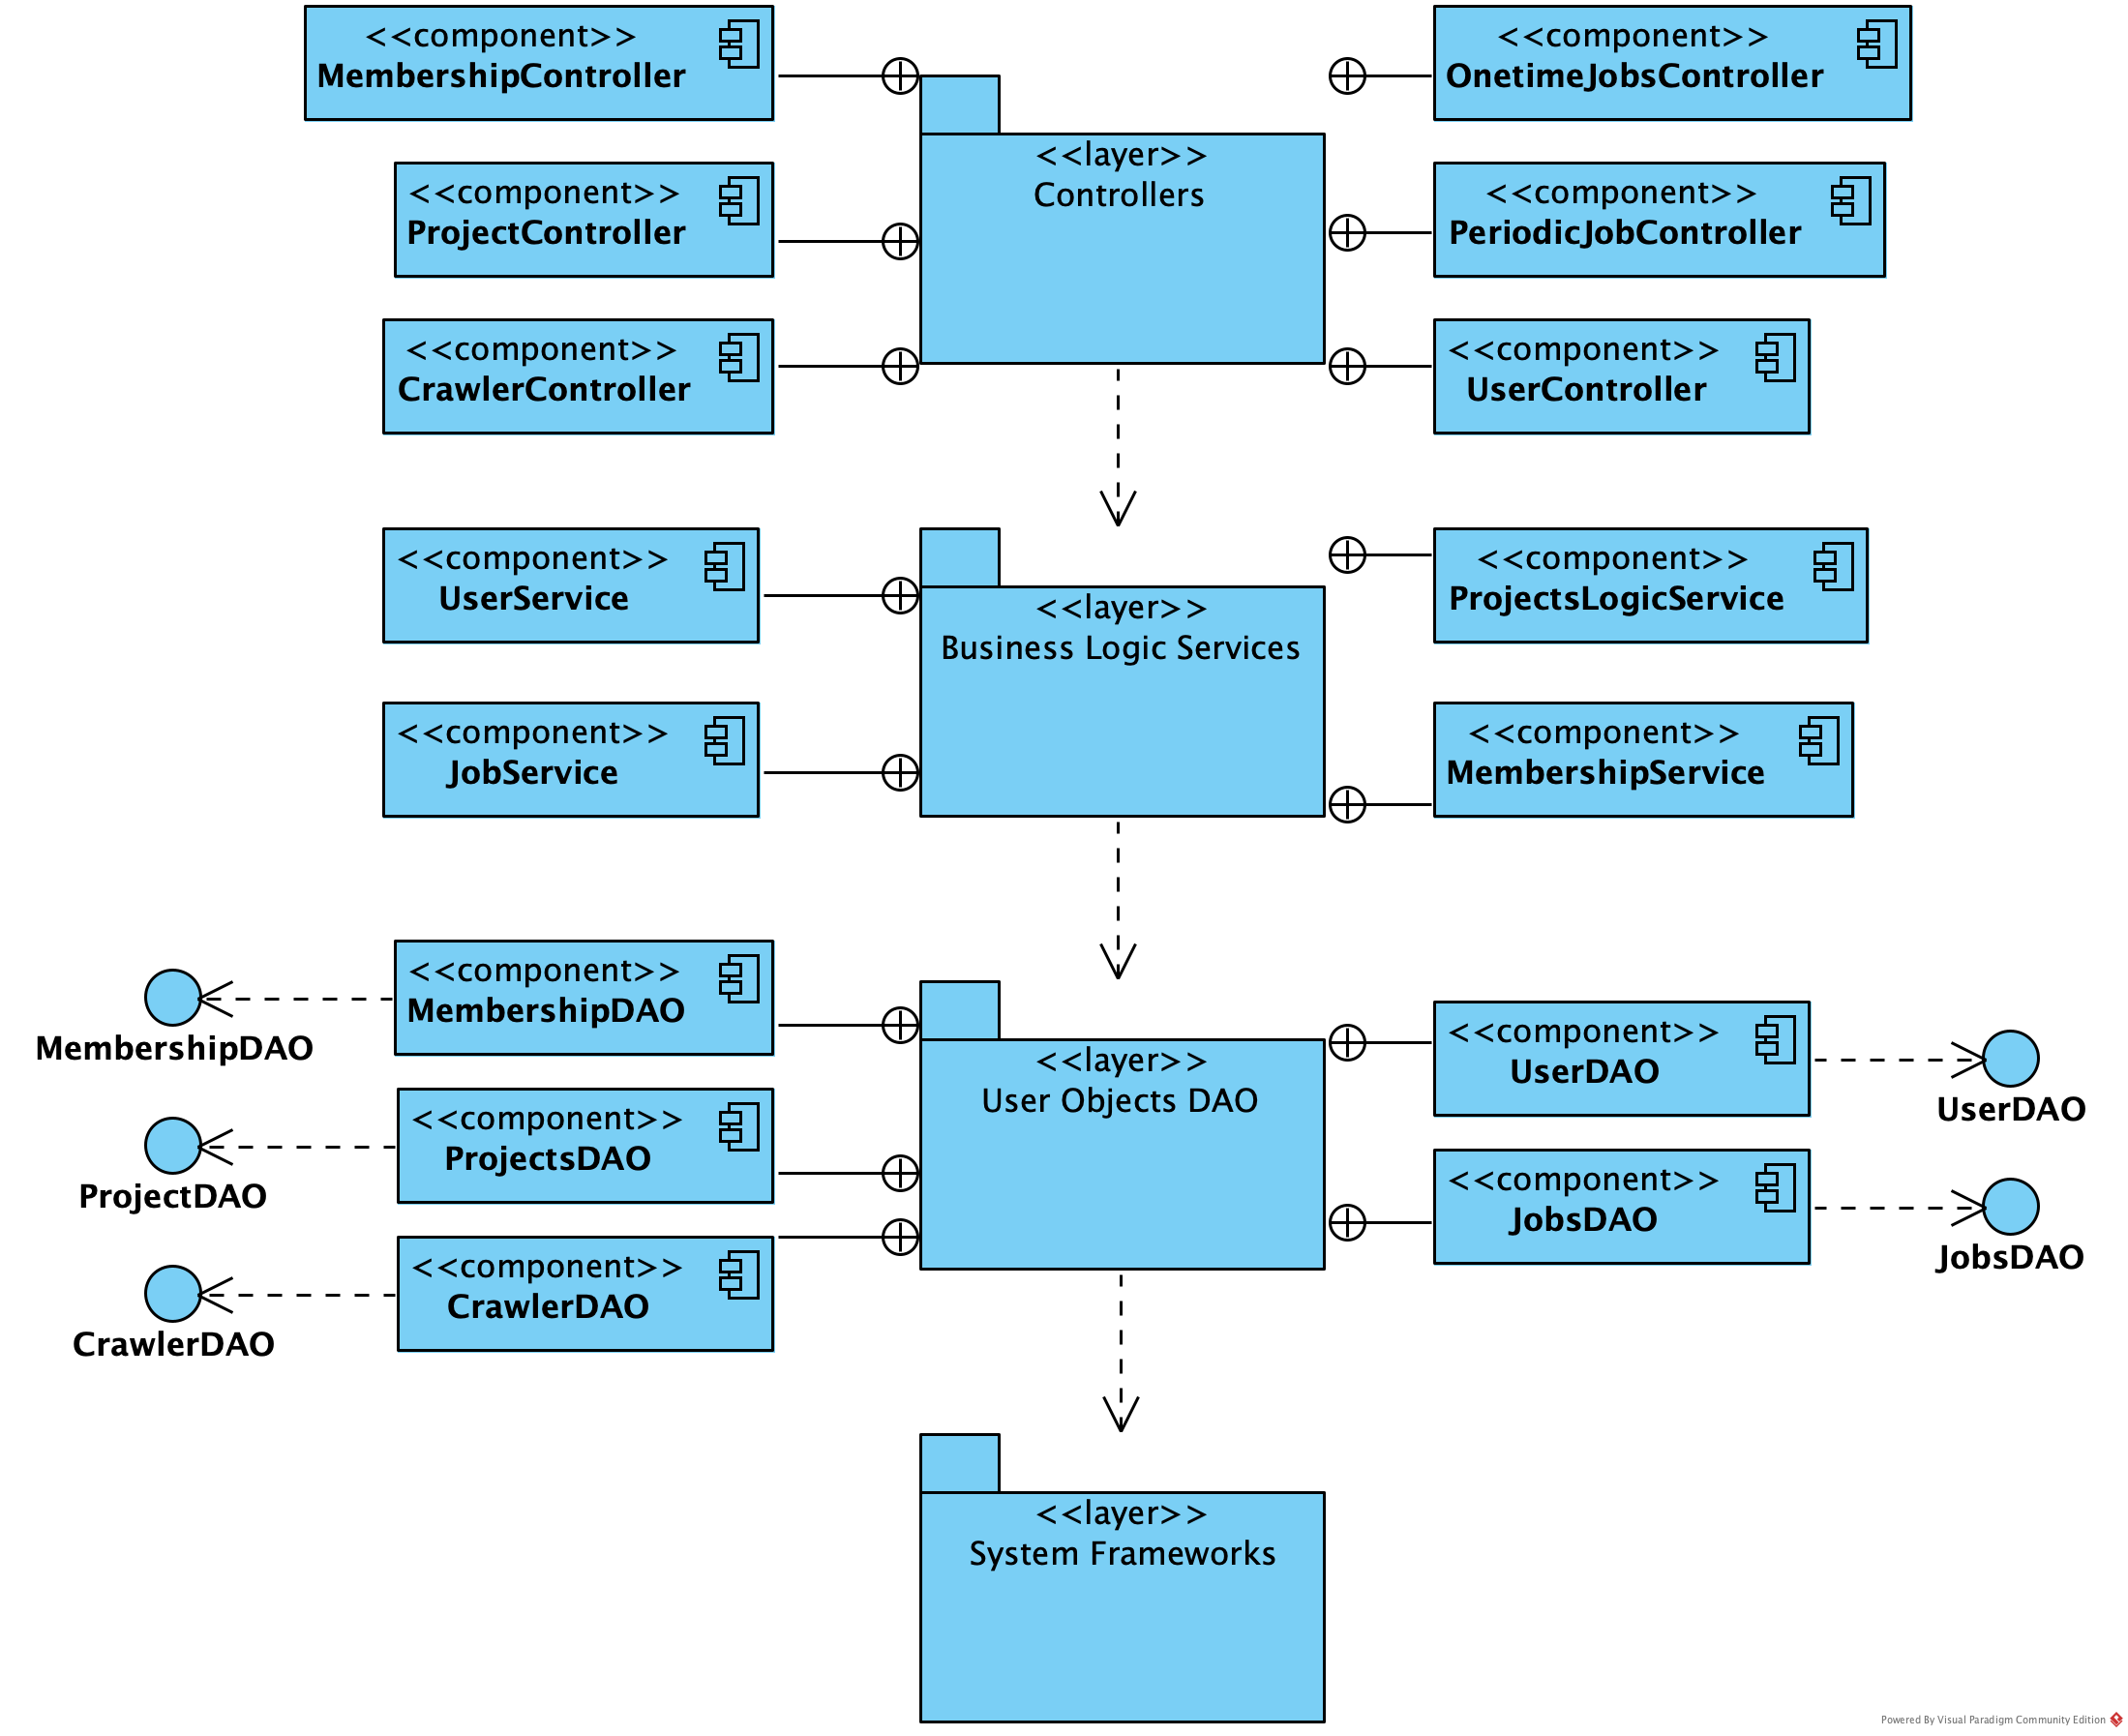
\includegraphics[width = 0.9\linewidth]{img/uml/ComponentDiagram.png}
		\caption{Пример слоистости в приложении}
		\label{pic:layers}
	\end{figure}
	
	\subsubsection{Обоснование выбора базы данных}
	\paragraph{PostgreSQL\\ \\}
	
	PostgreSQL\cite{postgresql} -- свободная объектно-реляционная система управления базами данных с открытым исходным кодом. 
    
    База данных позволяет хранить большое количество связанной и структурированной информации и эффективно производить манипуляции с ней. 
    
    Postgres также отличается хорошей поддержкой сериализации и индексации произвольных JSON~\cite{json} объектов, что сильно повышает гибкость в ее применении.

    Взаимодействие с базой данных производится на диалекте языка SQL. В рамках разработки большинство взаимодействия производилось посредством библиотеки play-slick (\cite{slick}) для строгой типизации и уменьшения ошибок со стороны программиста.
    
						\newpage
	\section{Технико-экономические показатели}
	\subsection{Предполагаемая потребность}
	\subsubsection{Устройство рынка}
	
	Рынок веб-скрейпинга составляют как коммерческие продукты, а также их open source аналоги. Web-scraping - это технология и методы, используемые стартапами, небольшими и крупными компаниями, которые делают возможным быстрое извлечение данных и информации из сети интернет и их обработку. Также технологии извлечения данных широко применяются в науке, образовании учебными, студентами и программистами.
	
	Таким образом, заинтересованных лиц на рынке выделить сложно - слишком большому кругу компаний сейчас требуется воспользоваться извлечением информации из интернета. Разрабатываемый продукт планируется сделать бесплатной площадкой для использования технологий web-scraping и доступной любому пользователю.
	
	\subsubsection{Пользовательская среда}
	
	Продукт будет применяться пользователями в рабочих, научных и исследовательских целях. Продуктом пользоваться можно будет как водиночку: запуск краулеров и сбор данных не требует дополнительных человеческих ресурсов, но также можно будет предоставлять доступ для наблюдения и редактирования запусков другим людям.
	
	Задачи, которые решают пользователи данной системой давольно обширные. Это может быть мелкая проблема, например как <<сбор данных о книгах с сайта>>, а вот примеры наиболее популярных крупных проблем:
	\begin{itemize}
		\item Сбор данных о продуктах и ценах для сравнения
		\item Сбор списков недвижимости
		\item Сбор данных для исследований
	\end{itemize}
	
	Перечисленный список задач компаниям и ученым приходится делать вручную или с использованием уже существующих аналогов - с этим они сталкиваются на регулярной основе. На данный момент существует много платных веб-сервисов, а также open source расширение для браузера.
	
	
	\subsubsection{Список пользователей} \label{subsub: userlist}
	\begin{table}[ht]
		\centering
		\begin{tabular}{|p{0.15\linewidth}|p{0.25\linewidth}|p{0.25\linewidth}|p{0.25\linewidth}|} 
			\hline
			\textbf{Роль пользователя продукта} & \textbf{Описание} & \textbf{Способ работы с продуктом} & \textbf{Представители
				интересов в процессе
				разработки}\\ \hline
			Обычный пользователь & Компания, заинтересованная в сборе данных; программист; студент; & Применение для сбора данных в учебных целях/ рабочих целях (мониторинг сайтов)/исследованиях & Представитель заказчика \\ \hline
		\end{tabular}
	\caption{Список пользователей}
	\end{table}

\newpage
	\subsubsection{Профили пользователей} \label{subsub: userprofile}
	
	\begin{table}[h!]
		\centering
		\begin{tabular}{|p{0.3\linewidth}|p{0.6\linewidth}|} 
			\hline
			\textbf{Категория пользователя} & \textit{Обычный пользователь} \\ \hline
			\textbf{Описание} & Пользователь, заинтересованный в сборе данных с помощью технологии web-scraping \\ \hline
			\textbf{Представители} & Компания, заинтересованная в сборе данных; стартап; программист; студент; научный сотрудник; аналитик \\ \hline
			\textbf{Уровень компетентности} & Определенный уровень знаний в области сбора данных и написании пауков для сбора данных, пользователь ПК \\ \hline
			\textbf{Обязанности} & 
			\begin{itemize}
				\item Использование продукта в целях сбора данных
				\item Мониторинг логов, ошибок
				\item Запуск периодических работ и мониторинг результатов
			\end{itemize}  \\ \hline
			\textbf{Критерий удовлетворенности продуктом} & Продукт удовлетворяет потребности в мониторинге и сборе данных \\ \hline
			\textbf{Степень вовлеченности} & Полная вовлеченность \\ \hline
			\textbf{Ожидаемые артифакты} & Логи, собранные данные \\ \hline
		\end{tabular}
		\caption{Профили пользователей}
	\end{table}
	\clearpage
	
	
	\subsubsection{Экономические преимущества по сравнению с отечественными и зарубежными аналогами}
	Система будет применяться как средство управления проектами по созданию, редактированию и запуску веб краулеров для сбора данных в сети интернет. Продукт позволит следить за запусками в режиме реального времени, а также создавать периодические запуски по расписанию.
 Разрабатываемая платформа предоставит бесплатный доступ к слудующему функционалу:
\begin{itemize}
    \item Совместное управление запусками клаулеров
    \item Периодический запуск задач
    \item Сбор логов, ошибок
    \item Группировка краулеров,а также их запусков в проект 
    \item Бесплатная функциональность
\end{itemize}
	
На рынке представлены следующие аналоги разрабатываемому планировщику заданий по запуску краулеров:
\subsection*{Системы с открытым исходным кодом}
\subsubsection*{scrapymon}

Простенький интерфейс для обзора задач и пауков над scrapyd. Нет поддержки планировщика. Нет дополнительного функционала, кроме базового запуска задач. Работает поверх scrapyd.

\subsubsection*{gerapy}

Работает поверх scrapyd. Api для запуска задач предоставляет cron-формат для периодического запуска. 

\subsubsection*{scrapydweb}

У продукта есть lgpl-лицензия, есть парсинг логов, удобный UI-интерфейс. Api для запуска задач предоставляет cron-формат для периодического запуска. Работает поверх scrapyd. 

\subsubsection*{ScrapyKeeper}

У продукта есть парсинг логов, удобный UI-интерфейс. Есть архивация версий и доступ к проектам. Api для запуска задач предоставляет cron-формат для периодического запуска. Работает поверх scrapyd. 

\subsection*{Проприетарные системы}

\subsubsection*{Scrapinghub.com}

Платная платформа, которая предоставляет возможность запускать периодические задачи, разрешает совместный доступ к проектам.


	\addition{Используемые понятия и определения}
	\begin{description}
		\item[\textbf{Web scraping}] -- это сбор данных с различных интернет-ресурсов. Общий принцип его работы можно объяснить следующим образом: некий автоматизированный код выполняет GET-запросы на целевой сайт и получая ответ, парсит HTML-документ, ищет данные и преобразует их в заданный формат. \label{terms:webscraping}
		\item[\textbf{Проект}] -- сущность для объединения и предоставления доступа к запускам/краулерам/периодическим задачам. \label{terms:project}
		
		\item[\textbf{Веб краулер}] --  программа, являющаяся составной частью поисковой системы и предназначенная для перебора страниц Интернета с целью занесения информации о них в базу данных поисковика. Неотъемлемая часть проекта. Именно с помощью пауков пользователь может “краулить” сайты для сбора необходимой информации. \label{terms:spider}
		\item[\textbf{Запуск}] -- единоразовый запуск краулера с настройками и аргументами, указанными для этого запуска. \label{terms:job}
		\item[\textbf{Периодический запуск}] -- запуск с множеством настроек, повторяющийся в определенные периоды времени (запуски по cron-expression).
		\label{terms:pjob}
	\end{description}
	
	\addition{Листинги}
	
	\begin{lstlisting}[frame=single, basicstyle=\footnotesize\ttfamily, label={lst:POST}, caption={JSON for POST /projects},captionpos=b]
{
    "name": "some name",
    "description": "optional description"
}
\end{lstlisting}


\begin{lstlisting}[frame=single, basicstyle=\footnotesize\ttfamily, label={lst:PUT}, caption={JSON for PUT /project},captionpos=b]
{
    "name": "some name",
    "description": "optional description",
    "spiderSettings": "{}",
    "spiderArgs": "{}"
}
\end{lstlisting}


\begin{lstlisting}[frame=single, basicstyle=\footnotesize\ttfamily, label={lst:DEPLOY}, caption={JSON for PUT /deploy},captionpos=b]
{
    "eggFile": <egg file>
}
\end{lstlisting}

\begin{lstlisting}[frame=single, basicstyle=\footnotesize\ttfamily, label={lst:POSTjob}, caption={JSON for POST /jobs},captionpos=b]
{
    "crawlerId": "CrawlerName",
    "priority": "Normal",
    "args": "{}",
    "settings": "{}"
}
\end{lstlisting}
	
	\addition{Описание классов, структур, методов, полей}
	
	\section*{Контроллеры}
	
	\begin{longtable}[]{|@{\textbf}r|p{7cm}|} 
	\hline
	ApplicationController.scala & API методы для доступа к авторизации \\ \hline
CrawlersController.scala & API методы для доступа к паукам \\ \hline
JobsController.scala & API методы для доступа к запускам \\ \hline
MembershipController.scala & API методы для доступа к участникам проекта \\ \hline
PeriodicJobsController.scala & API методы для доступа к периодическим запускам \\ \hline
ProjectsController.scala & API методы для доступа к проектам \\ \hline
SignInController.scala & API методы для доступа к авторизации \\ \hline
SignUpController.scala & API методы для доступа к регистрации \\ \hline
	
	\end{longtable}
	
	\section*{Сервисы}
	
	\begin{longtable}[]{|@{\textbf}r|p{7cm}|} 
	\hline
	JobService.scala & Сервис для управления запусками\\ \hline
MembershipService.scala & Сервис для управления\\ \hline
ProjectService.scala & Сервис для управления проектами\\ \hline
ScrapydService.scala & Сервис для отправки запросов в scrapyd \cite{scrapyd}\\ \hline
SecurityService.scala & Сервис для управления безопасностью доступа\\ \hline
UpdaterService.scala & Сервис для управления обновлениями и синхронизацией со scrapyd \cite{scrapyd}\\ \hline
UserService.scala & Сервис для управления пользователями\\ \hline

	\end{longtable}
	\section*{DAO}
	
	\begin{longtable}[]{|@{\textbf}r|p{7cm}|} 
	\hline
	CrawlersDAO.scala & Класс паук-объект базы данных\\ \hline
JobDAO.scala & Класс запуск-объект базы данных\\ \hline
MembershipDAO.scala & Класс участник-объект базы данных\\ \hline
PasswordDAO.scala & Класс пароль-объект базы данных\\ \hline
ProjectDAO.scala & Класс проект-объект базы данных\\ \hline
	\end{longtable}
						\newpage
	%\section{Источники, использованные при разработке}
	\renewcommand{\refname}{Список источников}
	\addcontentsline{toc}{section}{\refname}
	\begin{thebibliography}{7}
		\bibitem{scrapyd} Github scrapyd/scrapyd [Электронный ресурс] URL: \url{https://github.com/scrapy/scrapyd} (Дата обращения: 16.04.2020, режим доступа: свободный)
		\bibitem{gost}Единая система программной документации – М.: ИПК, Издательство стандартов, 2000, 125 стр.
		\bibitem{scalatestplus} ScalaTest+Play [Электронный ресурс] URL:\url{http://www.scalatest.org/plus}(Дата обращения: 16.04.2020, режим доступа: свободный)
		\bibitem{playsilhouettetestkit} Testing - silhouette [Электронный ресурс] URL:\url{https://www.silhouette.rocks/docs/testing} (Дата обращения: 16.04.2020, режим доступа: свободный)
		\bibitem{postgresql} Postgresql [Электронный ресурс] URL:\url{https://www.postgresql.org} (Дата обращения: 16.04.2020, режим доступа: свободный)
		
		\bibitem{flatmap} FlatMap [Электронный ресурс] URL:\url{https://www.scala-lang.org/api/current/scala/collection/View/FlatMap.html} (Дата обращения: 16.04.2020, режим доступа: свободный)
		
		\bibitem{json} JSON - Использование [Электронный ресурс]
		URL:\url{https://ru.wikipedia.org/wiki/JSON} (Дата обращения: 16.04.2020, режим доступа: свободный)
		
		\bibitem{silhouette} Silhouette - документация [Электронный ресурс] URL: \url{https://www.silhouette.rocks/docs} (Дата обращения: 16.04.2020, режим доступа: свободный)
		
		\bibitem{silhouette-testing} Silhouette-testing - документация [Электронный ресурс] URL: \url{https://www.silhouette.rocks/docs/testing} (Дата обращения: 16.04.2020, режим доступа: свободный)
		
		\bibitem{slick} Slick [Электронный ресурс] URL: \url{https://scala-slick.org}(Дата обращения: 16.04.2020, режим доступа: свободный)
		
		\bibitem{play} Play-framework [Электронный ресурс] URL:\url{https://www.playframework.com} (Дата обращения: 16.04.2020, режим доступа: свободный)
		
		\bibitem{play-mvc} Package play.mvc [Электронный ресурс] URL: \url{https://www.playframework.com/documentation/2.6.0/api/java/play/mvc/package-summary.html} (Дата обращения: 16.04.2020, режим доступа: свободный)
	\end{thebibliography}
	
						\newpage
	\listRegistration
	\addcontentsline{toc}{section}{Лист регистрации изменений}
\end{document} % конец документа